\chapter[Residues]{Evaluating Contour Integrals Using Residues}
\section{Motivation}
Let $\mathcal{C}$ be a simple, closed anticlockwise contour.  In the previous section we saw how certain integrals of the form
\[
\int_{\mathcal{C}} f
\]
may be calculated using Cauchy's Integral Formula, when $f$ is a function holomorphic on region $\mathcal{R} \backslash \set{z_0}$ with $z_0$ a point enclosed by $\mathcal{C}$.  However, this does not always work, as the following example illustrates.
\begin{example}
\label{e:gdef}
Cauchy's Integral Formula does not allow us to compute $\int_{\cont} f$, where $\mathcal{C}$ is the anticlockwise unit circle and $f$ is the function defined by
\[
f(z) = \frac{1}{z^2+\frac{1}{4}} = \frac{1}{(z+\frac{i}{2})(z-\frac{i}{2})},
\]
as there are two points enclosed by $\cont$ at which $f$ is not holomorphic. 
\begin{blankbox}
\begin{center}
\altgraphics[scale=1]{ch6_shrink1_full}{ch6_shrink1}
\end{center}
Draw the line $L=[-1,1]$ to get two new closed anticlockwise contours $\mathcal{C}_1$ and $\mathcal{C}_2$, with $\mathcal{C}_1$ enclosing $i/4$ and $\mathcal{C}_2$ enclosing $-i/4$.  Then
\[
\int_{\mathcal{C}} f = \int_{\mathcal{C}_1} f + \int_{\mathcal{C}_2} f,
\]
since the integral along $L$ in $\mathcal{C}_1$ and the integral along $\tilde{L}$ in $\mathcal{C}_2$ cancel.  We can then use Cauchy's Integral Formula to evaluate each of $\displaystyle \int_{\mathcal{C}_1} f$ and $\displaystyle \int_{\mathcal{C}_2} f$ separately.
\end{blankbox} 
\end{example}
We will assume without proof that the method we have just described will extend to the case when there is any finite number of points enclosed by $\mathcal{C}$ at which $f$ is not holomorphic:





\begin{theorem}[Generalised Shrinking Contour/ Deformation Theorem; proof non-examinable]
\label{t:gdef}
Let $\mathcal{R}$ be a simply connected region, $\mathcal{C}$ a simple, closed anticlockwise contour in $\mathcal{R}$, and $z_1,z_2,\ldots,z_n$ a finite collection of points that are enclosed by $\mathcal{C}$.  If $f$ is holomorphic on $\mathcal{R} \backslash \set{z_1,\ldots,z_n}$, then 
\[
\int_{\mathcal{C}} f = \int_{\mathcal{C}_1}f+ \ldots + \int_{\mathcal{C}_n} f,
\]
where each $\mathcal{C}_j$ is a closed simple anticlockwise circular contour enclosing $z_j$ and no other $z_k$.
\end{theorem}

\begin{figure}[H]
\centering
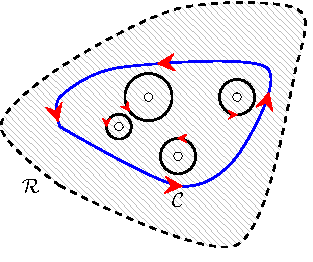
\includegraphics[scale=1]{ch6_residues2}
\caption{A contour $\mathcal{C}$ enclosing points $z_1,z_2,z_3$ and $z_4$ at which $f$ is not holomorphic.  The integral of $f$ along $\mathcal{C}$ is determined by the integrals along the circular contours enclosing these points.}
\end{figure}

 Theorem~\ref{t:gdef} allows us, as least in principle, to evaluate each $\int_{\mathcal{C}_j} f$ separately to obtain $\int_{\mathcal{C}} f$.  Thus we have essentially reduced the problem to that of evaluating integrals where there is one point enclosed by the given contour at which $f$ is not holomorphic.  
 
 This approach will not always work, however. 
  
\begin{example}
Let $f: \C \backslash \set{0} \to \C$ be defined by
\[
f(z) = \frac{\sin(z)}{z^2},
\]
and let $\mathcal{C}$ be any anticlockwise closed circular contour centred at $0$.
We cannot write
\[
\frac{\sin (z)}{z^2} = \frac{g(z)}{(z-z_0)}
\]
for any $z_0$ enclosed by $\mathcal{C}$ and $g$ holomorphic on a simply connected region containing $\mathcal{C}$.  Indeed the obvious choice would be to take $z_0=0$, but then we would have to define $g(z) = \dfrac{\sin(z)}{z}$, which still fails to be holomorphic on a suitable region.
\end{example}



\section{Singulairities of complex functions}
Theorem~\ref{t:gdef} shows that when calculating the integral of $f$ along a simple, anticlockwise, closed contour $\mathcal{C}$, the value $\int_{\mathcal{C}} f$ is in some sense depends only on those points at which $f$ is not holomorphic.  Therefore, we shall study these points in more detail.

\begin{definition}
A function $f$ has an \emph{isolated singularity} at the point $z_0$ if for some $r>0$, $f$ is holomorphic on a punctured disc $D'(z_0,r)$ but not on the (unpunctured) open disc $D(z_0,r)$.
\end{definition}
Note that if $f$ has an isolated singularity at $z_0$, it may be the case that $f$ is not defined at $z_0$, or $f$ is defined at $z_0$ but not differentiable there.

\begin{example}
The function $f$ defined by
\[
f(z) = \frac{1}{z^4+1}
\]
has isolated singularities at the points $e^{i\pi/4},\ e^{3i\pi/4},\ e^{5i\pi/4},\ e^{7i\pi/4}$; in each case, take $r = \frac{1}{4}$ for example.
\begin{center}
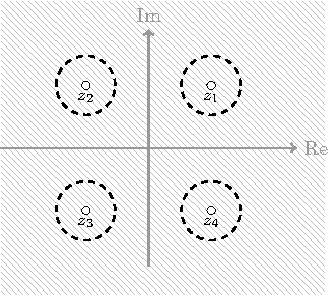
\includegraphics[scale=1]{ch6_poles1}
\end{center}
%\vspace*{2cm}

\end{example}
\begin{example}
The function $f$ defined by
\[
f(z) = \frac{\sin (z)}{z^2}
\]
has an isolated singularity at $0$.
\end{example}
\begin{example}
The Principal Logarithm function $\Log : \C \backslash \set{0}$ defined by
\[
\Log (z) = \log(\abs{z}) + i \Arg (z),
\]
is not holomorphic at any point on the negative real axis.  No such point is an isolated singularity of $\Log$
\end{example}
\begin{blankbox}
\begin{center}
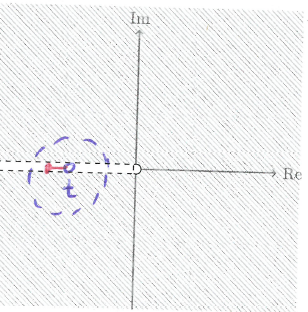
\includegraphics[scale=0.5]{ch6_non_iso_full}
\end{center}
Indeed, if $t \leq 0$ is a point on the negative real axis and $r>0$, then $D'(t,r)$ contains points at which $\Log$ is not holomorphic; $z=t-\frac{r}{2}$ for example.
%\vspace*{3cm}
\end{blankbox}
\begin{definition}  
Let $f$ be continuous on $\mathcal{R} \backslash \set{z_0}$. We say that $\displaystyle \lim_{z \to z_0} f(z) = \infty$ if given any $M>0$ there is some $r>0$ such that
\[
\abs{f(z)}>M \text{ for all } z \in D'(z_0,r).
\]
\end{definition}
\begin{example}

Consider the function
\[
f(z) = \frac{1}{(z-2i)^3}
\]
which has an isolated singularity at $2i$.  We will show that $\displaystyle \lim_{z \to 2i} f(z) = \infty$.
\end{example}
\begin{solution}

Indeed, given $M>0$, let $r=M^{-1/3}$.  Then 
\begin{align*}
0 < \abs{z-2i} < r \Rightarrow \abs{f(z)} &= \abs{\frac{1}{(z-2i)^3}}\\
& = \frac{1}{\abs{z-2i}^3} \\
& > \frac{1}{(M^{-1/3})^3} = M.
\end{align*}
\end{solution}
In most of the examples that we consider, $\displaystyle \lim_{z \to z_0} f(z) = \infty$ will occur whenever evaluating $f$ at $z_0$ would involve division by $0$ (except when $\frac{0}{0}$ would appear).  We shall make this more precise shortly.

\begin{definition}
A function $f$ with an isolated singularity $z_0$ is said to have a \emph{pole at $z_0$} if
\[
\lim_{z \to z_0} f(z) = \infty.
\]
Moreover, for $n \geq 1$, $f$ is said to have a \emph{pole of order $n$} at $z_0$ if for some $r>0$, $f$ can be represented in the form
\[
f(z) = \frac{g(z)}{(z-z_0)^n}\quad\text{ for all } z \in D'(z_0,r)
\]
where $g$ is holomorphic on $D(z_0,r)$ and $g(z_0) \neq 0$.
\end{definition}
Note that the representation
\[
f(z) = \frac{g(z)}{(z-z_0)^n}
\]
need not be valid everywhere on the domain of $f$, only inside the `small' disc $D(z_0,r)$.  The function $g$, unlike $f$, is both defined and differentiable at $z_0$.

\begin{example}
Let us return to the example of
\[
f(z) = \frac{1}{1+z^4}
\]
and investigate the pole $z_1 = e^{i\pi/4}$ of $f$.
\end{example}
\begin{solution}
Denote by $z_2,z_3$ and $z_4$ the other complex $4^{th}$ roots of $-1$, and let $g$ be the function defined by
\[
g(z) = \frac{1}{(z-z_2)(z-z_3)(z-z_4)}.
\]
Then $g$ is holomorphic on $\C \backslash \set{z_2,z_3,z_4}$, and in particular, holomorphic on $D(z_1,\frac{1}{2})$ for example (the precise value of $r>0$ is not important).
\begin{center}
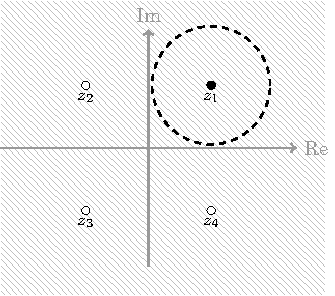
\includegraphics[scale=1]{ch6_poles2}
\end{center}
Moreover, $g(z_1) \neq 0$ and
\[
f(z) = \frac{g(z)}{z-z_1} \quad \text{ for all }\quad z \in D'(z_1,\tfrac{1}{2}).
\]
This shows that $f$ has a pole of order $1$ at $z_1$.
\end{solution}





%\vspace*{5cm}



\begin{example}
\label{e:poles2}
Let us investigate the poles of  the function
\[
f(z) = \frac{1}{(z^2+9)^2}.
\]
\end{example}
\begin{solution}
%\vspace*{12cm}
Using the factorisation
\[
z^2+9 = (z+3i)(z-3i)
\]
we have
\[
f(z)= \frac{1}{(z+3i)^2(z-3i)^2}
\]
so that $f$ has isolated singularities at $\pm 3i$.

If we define the function $g_1$ by
\[
g_1(z) = \frac{1}{(z+3i)^2}
\]
then $g_1$ is holomorphic on $\C \backslash \set{-3i}$ and in particular, holomorphic at $3i$ (that is, holomorphic on some open disc centred at $3i$, for example, $D(3i,1)$).  Since
\[
g_1(3i) = - \frac{1}{36} \neq 0 \quad\text{ and }\quad f(z) = \frac{g_1(z)}{(z-3i)^2} \quad\text{ for } z \in D'(3i,1)
\]
we see that $f$ has a pole of order $2$ at $z=3i$.

Similarly, by considering the function $g_2$ defined by
\[
g_2(z) = \frac{1}{(z-3i)^2}
\]
we see that $g_2$ is holomorphic and nonzero at $z=-3i$ and
\[
f(z) = \frac{g_2(z)}{(z+3i)^2}\quad\text{ for }\quad z \in D'(-3i,1)
\]
so that $f$ has a pole of order $2$ at $z=-3i$ also.
\end{solution}

%\newpage
\section{The Residue Theorem}

\begin{definition}
Let $f$ have an isolated singularity at $z_0$, then we define the \emph{residue of $f$ at $z_0$}, denoted by $\Res (f;z_0)$, to be
\[
\Res (f;z_0) = \frac{1}{2\pi i} \int_{\mathcal{C}} f
\]
where $\mathcal{C}$ is an anticlockwise simple closed contour which contains $z_0$ and no other singularities of $f$, and lies inside a region in which $f$ is holomorphic.
\end{definition}
If $f$ has an isolated singularity at $z_0$, then such a contour $\mathcal{C}$ can always be found.  Indeed, we know that $f$ is holomorphic on the punctured disc $D'(z_0,r)$ for some $r>0$.  Thus we may take $\mathcal{C}$ to be the anticlockwise circle with centre $z_0$ and radius $r/2$.


For example, we have seen before that with $\mathcal{C}$ the anticlockwise unit circle,
\[
\int_{\mathcal{C}} \frac{1}{z}\ dz=2\pi i \quad \text{ and} \quad \int_{\mathcal{C}} \frac{1}{z^2}\ dz = 0.
\]
Thus for the functions $f$ and $g$ defined by $f(z)=\dfrac{1}{z}$ and $g(z) = \dfrac{1}{z^2}$ we have
\[
\Res (f;0)=1 \quad \text{ and } \quad \Res (g;0) = 0.
\]
%\vspace*{7cm}


Theorem~\ref{t:residue} is essentially a reformulation of the Generalised Deformation Theorem (Theorem~\ref{t:gdef}), and generalises Cauchy's Integral Formula.
\begin{theorem}[The Residue Theorem]
\label{t:residue}
Let $\mathcal{R}$ be a simply connected region and let $f$ be a function that is holomorphic on the region $\mathcal{R} \backslash \set{ z_1,z_2,\ldots , z_n}$ and has isolated singularities at the points $z_1,z_2,\ldots,z_n$. If $\mathcal{C}$ is an anticlockwise simple closed contour that lies in $\mathcal{R}\backslash \set{z_1,z_2,\ldots,z_n}$ and encloses the points $z_1,z_2,\ldots,z_n$, then
\[
\int_{\mathcal{C}} f = 2 \pi i \left( \Res (f;z_1)+\Res (f;z_2) + \ldots + \Res (f;z_n ) \right).
\]
\end{theorem}
In other words
\[
\int_{\mathcal{C}} f = 2\pi i \left( \text{ sum of residues of $f$ at isolated singularities enclosed by $\mathcal{C}$ } \right)
\]

\begin{figure}[H]
\centering
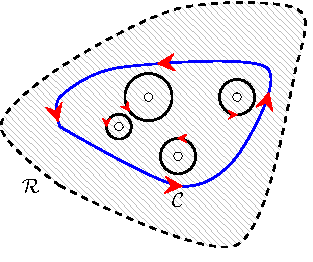
\includegraphics[scale=1]{ch6_residues2}
\caption{At each singularity $z_j$, the residue of $f$ at $z_j$ is given by the the integral of $f$ along the small circular contour surrounding $z_j$ (divided by $2\pi i$).  The integral of $f$ along $\mathcal{C}$ is then determined by these residues.}
\end{figure}

We want to use the Residue Theorem to evaluate contour integrals.  The theorem may not look particularly useful yet, since residues themselves are defined to be integrals along circular contours.  However, the following two theorems show us that certain residues may be calculated without performing any integration.




We will need the following Lemma, the proof of which is omitted.
\begin{lemma}[Proof non-examinable]
\label{l:goverh}
Suppose that $z_0 \in \C$, $h$ is holomorphic at the point $z_0$ with $h(z_0)=0$ and $h'(z_0) \neq 0$.  Then there is some $\delta>0$ and a holomophic function $k:D(z_0,\delta) \to \C$ with $k(z) \neq 0$ and $h(z)=(z-z_0)k(z)$ for all $z \in D(z_0,\delta)$.
\end{lemma}
\begin{theorem}[The $g/h$ rule]
\label{t:goverh}
Let $z_0 \in \C,\ r>0$ and let $f$ be holomorphic on $D'(z_0,r)$. Suppose that $f$ can be represented by
\[
f(z) = \frac{g(z)}{h(z)}\quad \text{ for } z \in D'(z_0,r)
\]
where $g$ and $h$ are holomorphic on $D(z_0,r)$, and $g(z_0) \neq 0$, $h(z_0)=0$ and $h'(z_0) \neq 0$. Then
\begin{enumerate}
\item[(i)] The function $f$ has an isolated singularity, and in particular, a  pole of order one at $z_0$.
\item[(iii)] The residue of $f$ at $z_0$ is given by
\[
\Res (f,z_0) = \frac{g(z_0)}{h'(z_0)}.
\]
\end{enumerate}
\end{theorem}
\begin{proof}
By Lemma~\ref{l:goverh} we obtain $\delta>0$ (making $\delta<r$ if necessary) and $k:D(z_0,\delta)\to \C$, with $k$ holomorphic and nonzero on $D(z_0,\delta)$ and
\[
f(z)= \frac{g(z)}{k(z)}\cdot \frac{1}{(z-z_0)} \quad \text{ for all } z \in D'(z_0,\delta).
\]
Since $k(z) \neq 0$ for all $z \in D(z_0,\delta)$ the function $z \mapsto \frac{g(z)}{k(z)}$ is holomorphic on $D(z_0,\delta)$, and since $g(z_0) \neq 0$, $f$ has a pole of order $1$ at $z_0$.

If $\mathcal{C}$ is the anticlockwise circle with centre $z_0$ and radius $r/2$, then Cauchy's Integral Formula gives
\[
\Res (f;z_0) = \frac{1}{2\pi i} \int_{\mathcal{C}} f = \frac{1}{2\pi i} \int_{\mathcal{C}} \frac{g(z)}{k(z)} \cdot \frac{1}{z-z_0}\ dz = \frac{g(z_0)}{k(z_0)}.
\]
But then by the product rule, $h'(z) = k(z)+(z-z_0)k'(z)$ for all $z \in D(z_0,\delta)$, so that $h'(z_0) = k(z_0)$, thus
\[
\Res (f;z_0) = \frac{g(z_0)}{h'(z_0)}.
\]
\end{proof}



\begin{example}
Let us calculate the residues at the poles of the function $f$ defined by
\[
f(z) = \frac{1}{1+z^2}.
\]
\end{example}
\begin{solution}
%\vspace*{12cm}
With $g(z)=1$ and $h(z)=1+z^2$, we have $h(z)=0$ at $z=\pm i$, and $h'(z)=2z \neq 0$ at these points.
Hence $f$ has poles of order $1$ at $z=\pm 1$, with residues
\begin{align*}
\Res (f;i ) & = \frac{g(i)}{h'(i)} = \frac{1}{2i} = - \frac{i}{2} \\
\Res (f;-i) & = \frac{g(-i)}{h'(-i)} = \frac{1}{-2i} = \frac{i}{2}.
\end{align*}

Consider the simple, closed anticlockwise contours $\mathcal{C}_1,\mathcal{C}_2$ and $\mathcal{C}_3$ shown below.
\begin{center}
\begin{tabular}{ccc}
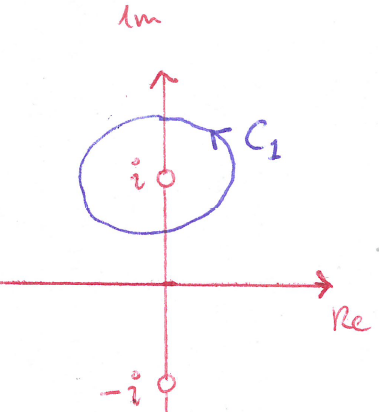
\includegraphics[scale=0.45]{ch6_res1full} & 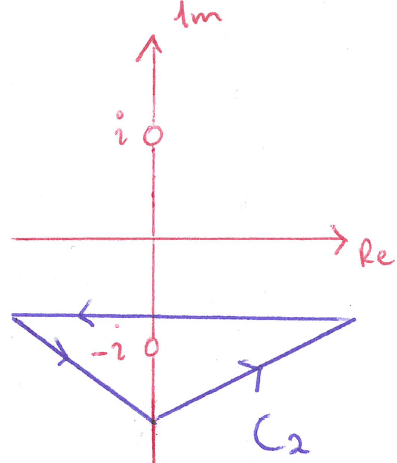
\includegraphics[scale=0.45]{ch6_res2full} & 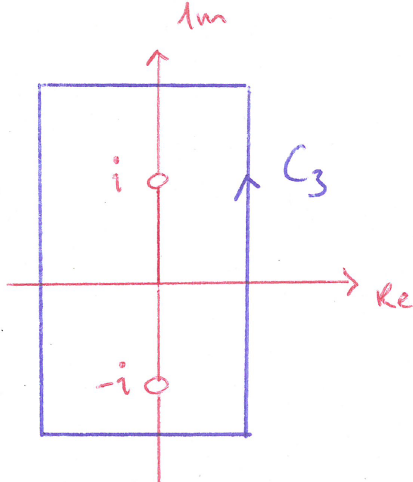
\includegraphics[scale=0.45]{ch6_res3full}
\end{tabular}
\end{center}
By the Residue Theorem, we have
\begin{align*}
\int_{\mathcal{C}_1} f &= 2\pi i \left[ \Res (f;i) \right] = 2\pi i \left[ \frac{-i}{2} \right] = \pi \\
\int_{\mathcal{C}_2} f &= 2\pi i \left[ \Res (f;-i) \right] =2\pi i \left[ \frac{i}{2} \right] = -\pi\\
\int_{\mathcal{C}_3} f &= 2\pi i \left[ \Res (f;i)+\Res(f;-i) \right] = 2\pi i \left[ -\frac{i}{2} + \frac{i}{2} \right] = 0,
\end{align*}
since $\mathcal{C}_1$ encloses the singularity $z=i$ and no others, $\mathcal{C}_2$ encloses the singularity $z=-i$ and no others, and $\mathcal{C}_3$ encloses the singularities $z=i$ and $z=-i$.
\end{solution}
\begin{example}
Let us do the same for the function
\[
f(z) = \frac{-i}{6z^2+13z+6}
\]
\end{example}
\begin{solution}
Let $g(z)=-i$ and 
\[
h(z) = 6z^2+13z+6 = (3z+2)(2z+3)
\]
and note that $h(z)=0$ for $z=-\frac{2}{3},-\frac{3}{2}$.  Since $h'(z)=12z+13$, we have
\[
h'(-2/3)  = 5 \quad\text{ and}\quad h'(-3/2) = -5,
\]
both of which are nonzero, so that $f$ has poles of order $1$ at $-\frac{2}{3}$ and $-\frac{3}{2}$ by Theorem~\ref{t:goverh}.  Moreover, by the same result,
\begin{align*}
\Res(f;-2/3) & = \frac{g(-2/3)}{h'(-2/3)} = - \frac{i}{5} \\
\Res (f;-3/2) & = \frac{g(-3/2)}{h'(-3/2)} = \frac{i}{5}.
\end{align*}
\end{solution}
%\vspace*{20cm}
%\begin{absolutelynopagebreak}
\begin{theorem}[The Residue at a pole of order $n$]
\label{t:polen}
Let $f$ have an isolated singularity at $z_0$ which is a pole of order $n$, so that for some $r>0$
\[
f(z) = \frac{g(z)}{(z-z_0)^n} \quad \text{ for } z \in D'(z_0,r),
\]
with $g$ holomorphic on $D(z_0,r)$ and $g(z_0) \neq 0$.  Then
\[
\Res (f,z_0) = \frac{g^{(n-1)}(z_0)}{(n-1)!}.
\]
\end{theorem}
%\end{absolutelynopagebreak}
%\noindent\textit{Proof:}
\begin{proof}
By definition,
\[
\Res (f;z_0) = \frac{1}{2\pi i} \int_{\mathcal{C}} \frac{g(z)}{(z-z_0)^n}\ dz,
\]
where $\mathcal{C}$ is the anticlockwise circle with centre $z_0$ and radius $r/2$.  By Theorem~\ref{t:cauchyd} (Cauchy's Integral Formula for Derivatives),
\[
g^{(n-1)} (z_0) = \frac{(n-1)!}{2\pi i} \int_{\mathcal{C}} \frac{g(z)}{(z-z_0)^n}\ dz,
\]
so that
\[
g^{(n-1)} (z_0) = (n-1)!\ \Res (f;z_0),
\]
or in other words,
\[
\Res (f;z_0) = \frac{g^{(n-1)}(z_0)}{(n-1)!}.
\]
\end{proof}
%\vspace*{10cm}



\begin{example}
\label{e:res3}
%\begin{absolutelynopagebreak}
Let us consider the function $f$ defined by
\[
f(z) = \frac{1}{(z^2+9)^2}.
\]
and calculate the residues at the poles of $f$.
\end{example}
\begin{solution}
%\end{absolutelynopagebreak}
Following Example~\ref{e:poles2}, we define $g_1$ and $g_2$ by
\[
g_1(z) = \frac{1}{(z+3i)^2} \quad\text{ and }\quad g_2(z) = \frac{1}{(z-3i)^2}
\]
so that
\[
f(z) = \frac{g_1(z)}{(z-3i)^2} = \frac{g_2(z)}{(z+3i)^2},
\]
and $g_1$ is holomorphic and nonzero at $z=3i$, $g_2$ is holomorphic and nonzero at $z=-3i$.  

Since the poles at $z=\pm 3i$ both have order $2$, Theorem~\ref{t:polen} tells us that
\[
\Res (f;3i) =\frac{g_1'(3i)}{1!} \quad\text{ and } \Res (f;-3i) = \frac{g_2'(-3i)}{1!}.
\]
The required derivatives are
\begin{align*}
g_1'(z) = -2(z+3i)^{-3} & \Rightarrow g_1'(3i) = -2(3i+3i)^{-3} = - \frac{i}{108} \\
g_2'(z) = -2(z-3i)^{-3} & \Rightarrow g_2'(-3i) = -2(-3i-3i)^{-3} = \frac{i}{108},
\end{align*}
Hence
\[
\Res (f;3i) = \frac{-i/108}{1!} = - \frac{i}{108} \quad\text{ and }\quad \Res (f;-3i) = \frac{i/108}{1!}= \frac{i}{108}.
\]
%\vspace*{15cm}

\end{solution}

\begin{example}
%\begin{absolutelynopagebreak}
For the function $f$ defined by
\[
f(z) = \frac{\exp(\pi z)}{(z-i)^3}
\]
find $\Res (f,i)$.  Hence evaluate
\[
\int_{\mathcal{C}} \frac{\exp( \pi z)}{(z-i)^3}\ dz,
\]
where $\mathcal{C}$ is the anticlockwise triangular contour with vertices $2$, $2i$ and $-2$.
\end{example}
%\end{absolutelynopagebreak}
%\vspace*{15cm}
\begin{solution}
The only pole of $f$ is a pole of order $3$ at $z=i$.  With $g$ the holomorphic function defined by $g(z) = \exp(\pi z )$, we have $g'(z) = \pi \exp(\pi z)$ and $g''(z) = \pi^2 \exp(\pi z)$.  By Theorem~\ref{t:polen},
\[
\Res(f;i) = \frac{g''(i)}{2!} = \frac{\pi^2 \exp(\pi i)}{2!} = \frac{\pi^2(-1)}{2} = - \frac{\pi^2}{2}.
\]
Since $\mathcal{C}$ is a simple, closed anticlcokwise contour, and $i$ is the only pole of $f$ enclosed by $\mathcal{C}$, the Residue Theorem gives
\[
\int_{\mathcal{C}} f = 2\pi i \Res (f;i) = 2\pi i \left( -\frac{\pi^2}{2} \right) = -i \pi^3.
\]
\end{solution}

%\newpage
\section{Evaluating Real Integrals using Contour Integration, part 2}
Recall how we used contour integration to evaluate
\[
\int_{-\infty}^{+\infty} \frac{1}{1+x^2}\ dx.
\]
We first considered the complex function $f$ where $f(z)=\dfrac{1}{1+z^2}$, and computed the integral of $f$ along the path $\cont_R = L_R+S_R$ consisting of the line segment $[-R,R]$ and the upper semicircle with centre $0$ and radius $R$, from $R$ to $-R$ via $iR$ (where $R>1$).

We did this using Cauchy's Integral Formula, though we could equally have used the Residue Theorem.  We then showed that
\[
\lim_{R \to \infty} \int_{S_R} f = 0
\]
using The Estimation Lemma.  From this we deduced that
\[
\int_{-\infty}^{+\infty} \frac{1}{1+x^2}\ dx  = \lim_{R \to \infty} \int_{L_R} f = \lim_{R \to \infty} \left( \int_{L_R}f + \int_{S_R} f \right)
= \int_{\cont_R} f. 
\]
In fact, the exact same method can be used to evaluate many integrals of the form
\[
\int_{-\infty}^{+\infty} f(x)\ dx,\quad\text{ for example}\quad \int_{-\infty}^{+\infty} \frac{p(x)}{q(x)}\ dx
\]
with $p$ and $q$ real polynomials, where $q$ has no real roots and the degree of $q$ is at least the degree of $p$ plus 2.
\begin{example}
\label{e:realint2}
Let us evaluate
\[
\int_{-\infty}^{+\infty} \frac{1}{(x^2+9)^2}\ dx
\]
using contour integration.
\end{example}
\begin{solution}

We shall follow the approach used in Example~\ref{e:realint1}, by considering the complex function $f$ defined via
\[
f(z) = \frac{1}{(z^2+9)^2}
\]
and the contour $\mathcal{C}_R=L_R+S_R$, where $R>3$, $L_R=[-R,R]$ and $S_R$ is the upper semicircle with centre $0$ and radius $R$ from $R$ to $-R$ via $iR$.

Using the result of Example~\ref{e:res3}, the only singularity of $f$ enclosed by $\mathcal{C}_R$ is at $z=3i$, hence by the Residue Theorem
\[
\int_{\mathcal{C}_R} f = 2\pi i \Res (f;3i) = 2\pi i \left( -\frac{i}{108} \right) = \frac{\pi}{54}
\]
for all $R>3$.

If $z \in S_R$, then $\abs{z}=R$ and hence by the reverse triangle inequality
\[
\abs{z^2+9} \geq \abs{\abs{z^2}-9} = \abs{\abs{z}^2-9} = R^2-9,
\]
so that for all such $z$ we have $\abs{z^2+9}^2 \geq \left( R^2-9 \right)^2$.  Thus for all $z \in S_R$,
\[
\abs{\frac{1}{(z^2+9)^2}} = \frac{1}{\abs{z^2+9}^2} \leq \frac{1}{\left(R^2-9 \right)^2}.
\]
The Estimation Lemma gives
\[
\abs{ \int_{\mathcal{C}_R} \frac{1}{(z^2+9)^2}\ dz } \leq \frac{1}{\left(R^2-9 \right)^2} \cdot \pi R,
\]
hence $\displaystyle \int_{\mathcal{C}_R} f \to 0$ as $R \to \infty$ as before.

Parameterising $L_R$ using $\gamma:[-R,R] \to \C$, $\gamma(t)=t$ we have $\gamma'(t)=1$ and so
\[
\int_{L_R} f = \int_{-R}^{R} \frac{1}{(t^2+9)^2}\ dt.
\]
Hence
\begin{align*}
\frac{\pi}{54} & = \int_{\mathcal{C}_R} f  && (\forall\ R>3) \\
& = \lim_{R \to \infty} \int_{\mathcal{C}_R} f && \\
& = \lim_{R \to \infty} \left( \int_{L_R} f \right) + \lim_{R \to \infty} \left( \int_{S_R} f \right) && \\
& = \lim_{R \to \infty} \int_{-R}^{+R} \frac{1}{(t^2+9)^2}\ dt\ +0&& \\
 &= \int_{-\infty}^{+\infty} \frac{1}{(t^2+9)^2}\ dt. &&
\end{align*}
(Note that it does not matter whether we call the variable of integration $x$ or $t$).
\end{solution}
\begin{example}
Use Example~\ref{e:realint2} to deduce the value of
\[
\int_0^{\infty} \frac{1}{(x^2+9)^2}\ dx.
\]
\end{example}
\begin{solution}
Since $\displaystyle f(x) = \frac{1}{x^2+9}$ is an even function (i.e. $f(-x)=f(x)$) it follows that
\[
\int_0^{\infty} \frac{1}{(x^2+9)^2}\ dx  = \frac{1}{2} \int_{-\infty}^{\infty} \frac{1}{(x^2+9)^2}\ dx = \frac{\pi}{108}.
\]
\end{solution}


We showed in example~\ref{e:trig2} that for a rational function $R$ of two real variables
\[
\int_0^{2\pi} R ( \cos(t), \sin(t))\ dt = \int_{\mathcal{C}} R \left( \frac{z+z^{-1}}{2} , \frac{z-z^{-1}}{2i} \right) \cdot \frac{1}{iz}\ dz
\]
where $\mathcal{C}$ is the anticlockwise circle $\set{z \in \C: \abs{z}=1}$.

\begin{example}
Evaluate
\[
\int_0^{2\pi} \frac{\sin (t)}{5-4\sin(t)}\ dt
\]
using contour integration.
\end{example}
\begin{solution}
For $z = \exp (it) \in \mathcal{C}$, define $f$ via 
\begin{align*}
f(z) = R \left( (z+z^{-1})/2,(z-z^{-1})/(2i) \right) \cdot \frac{1}{iz}\ & = \frac{[z-z^{-1}]/(2i)}{5-4[z-z^{-1}]/(2i)}\cdot \frac{1}{iz} \\
& = \frac{z-z^{-1}}{10i-4z+4z^{-1}} \cdot \frac{1}{iz} \\
& =  \frac{z^2-1}{-4z^2+10iz+4} \cdot \frac{1}{iz} \\
& =  \frac{i(z^2-1)}{z(4z^2-10iz-4)}\\
& = \frac{1}{2} \cdot \frac{i(z^2-1)}{z(z-2i)(2z-i)}
\end{align*}
so that
\[
\int_0^{2\pi} \frac{\sin (t)}{5-4\cos(t)}\ dt = \int_{\mathcal{C}}  f dz.
\]
The function $f$ has simple poles at $0, i/2$ and $2i$, and  the first two of these are enclosed by $\mathcal{C}$.  Writing
\[
g(z)=i(z^2-1) \quad \text{ and } h(z) = 4z^3-10iz^2-4z
\]
we have $f=g/h$ and $h'(z)=12z^2-20iz-4$, hence by the $g/h$ rule
\begin{align*}
\mathrm{Res} (f;0) & = \frac{g(0)}{h'(0)} = \frac{-i}{-4} = \frac{i}{4} \\
\mathrm{Res} (f;i/2) & = \frac{g(i/2)}{h'(i/2)} = \frac{i((\tfrac{i}{2})^2-1)}{12(\tfrac{i}{2})^2-20i(\tfrac{i}{2})-4} =\frac{-5i}{12}.
\end{align*}
The Residue Theorem gives 
\[
\int_{\mathcal{C}}  \frac{(z^2-1)}{2z(z-2i)(2z-i)}\ dz =  2 \pi i \left( \frac{i}{4} - \frac{5i}{12} \right) =2\pi i \left(\frac{-i}{6} \right) = \frac{\pi}{3}. 
\]
Hence
\[
\int_0^{2\pi} \frac{\sin (t)}{5-4\sin(t)}\ dt =\frac{\pi}{3}.
\]
\end{solution}








